\chapter{Caches}
\section{Why Caches}
The difference between cycle time (time of a stage in a pipeline) and memory access time has continually increased.
\begin{center}
    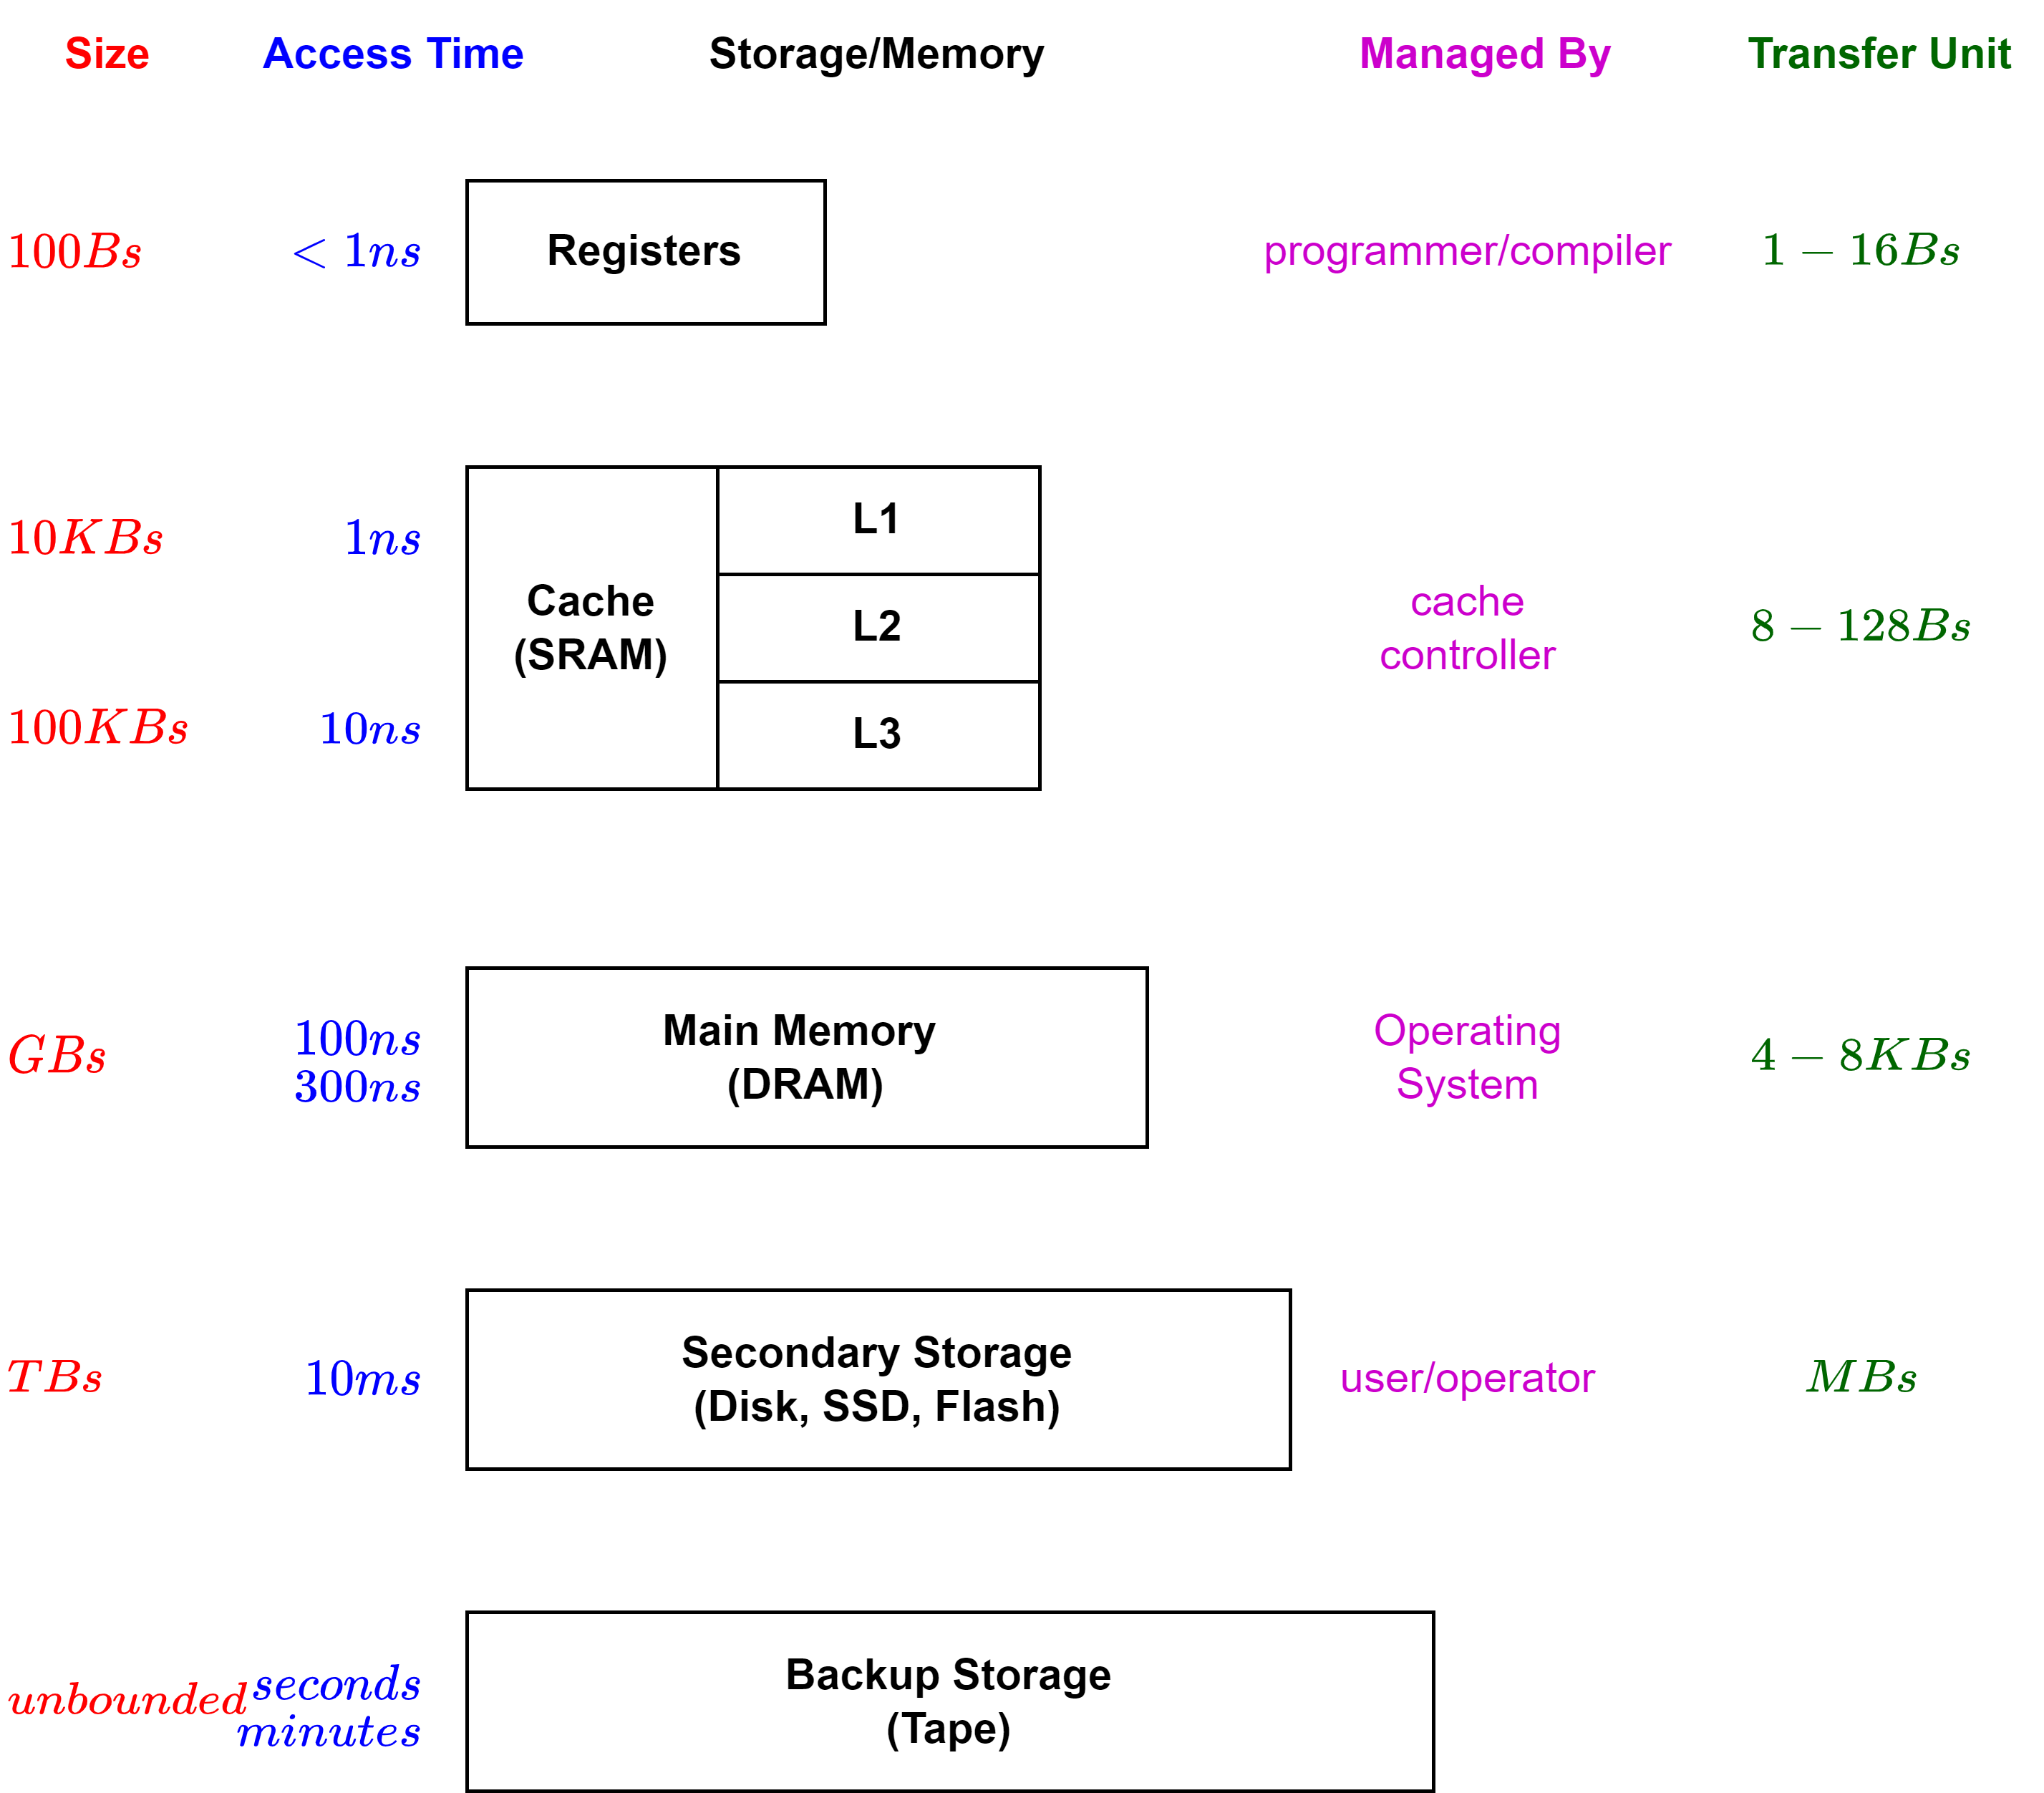
\includegraphics[width=.9\textwidth]{caches/images/memory_hierarchy.drawio.png}
\end{center}
\section{Locality}
Programs typically access only a small part of their address space during a short time period.
\begin{tcbraster}[raster columns=2,raster equal height]
    \begin{definitionbox}{Temporal Locality}
        Locality in time. The same location referenced is often referenced multiple times.
    \end{definitionbox}
    \begin{definitionbox}{Temporal Locality}
        Locality in space. Locations near an accessed location tend to be referenced soon.
    \end{definitionbox}
\end{tcbraster}
Most modern architectures are reliant on locality to determine when and what locations should be cached.
\begin{itemize}
    \item Cache is a scarce resource.
    \item Cache misses are expensive.
\end{itemize}

\section{Cache Types}
\subsection{Directly Mapped Cache}
\begin{definitionbox}{Associativity Conflicts}
    Where two or more locations are mapped to the same cache line/set of cache lines, and repeatedly replace each other.
    \begin{minted}{C}
/* Example with arrays, assume cache line is 256 bytes
 * and both arrays start at same cache index 
 */

int array_a[64];
int array_b[64];

int some_function() {
    int sum = 0;
    for (int i = 0; i < 64; i++) {
        r += 
        array_a[i]    /* array_a moved into cache line */
        + array_b[i]; /* array_b evicts array_a and replaces */
    }
    return sum;
}
    \end{minted}
\end{definitionbox}

\begin{center}
    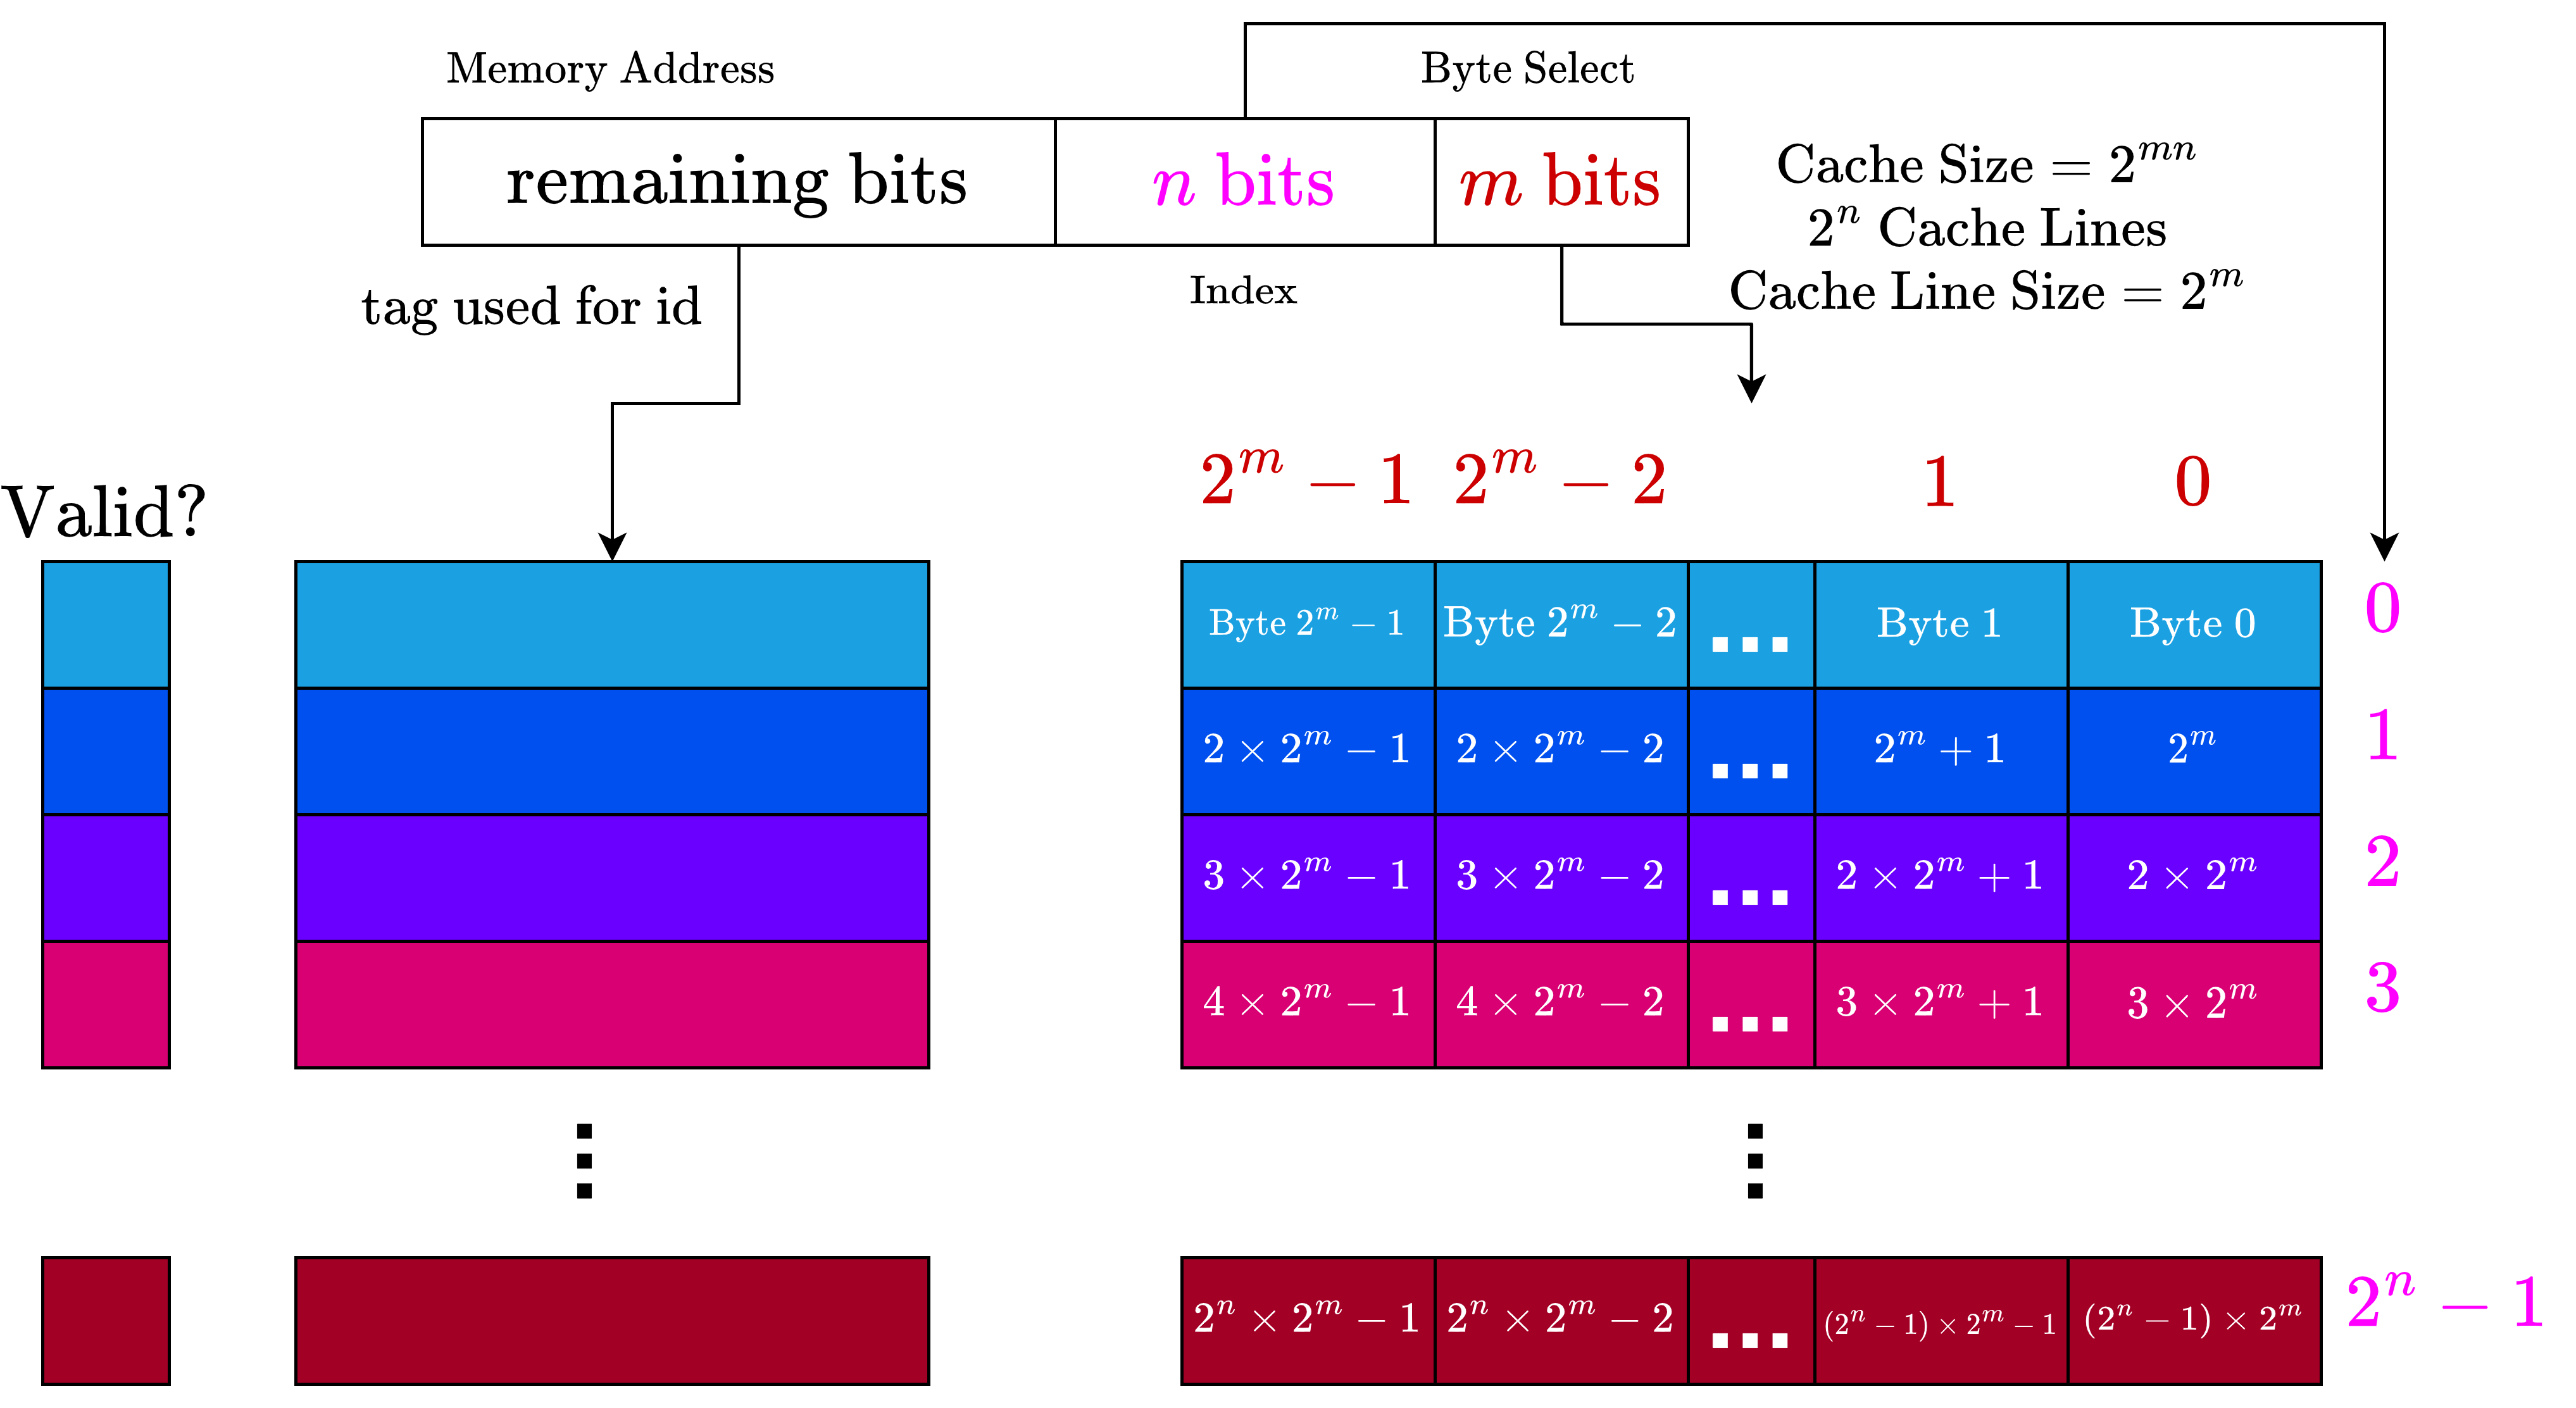
\includegraphics[width=.9\textwidth]{caches/images/direct_mapped_cache.drawio.png}
\end{center}
\begin{itemize}
    \item Index and byte select used to find entry. Then tag compared to determine hit/miss.
    \item We can see a pattern in memory of where locations can be cached based on the index.
    \item Block/line received before the hit/miss is known (recover later if miss).
\end{itemize}
\begin{center}
    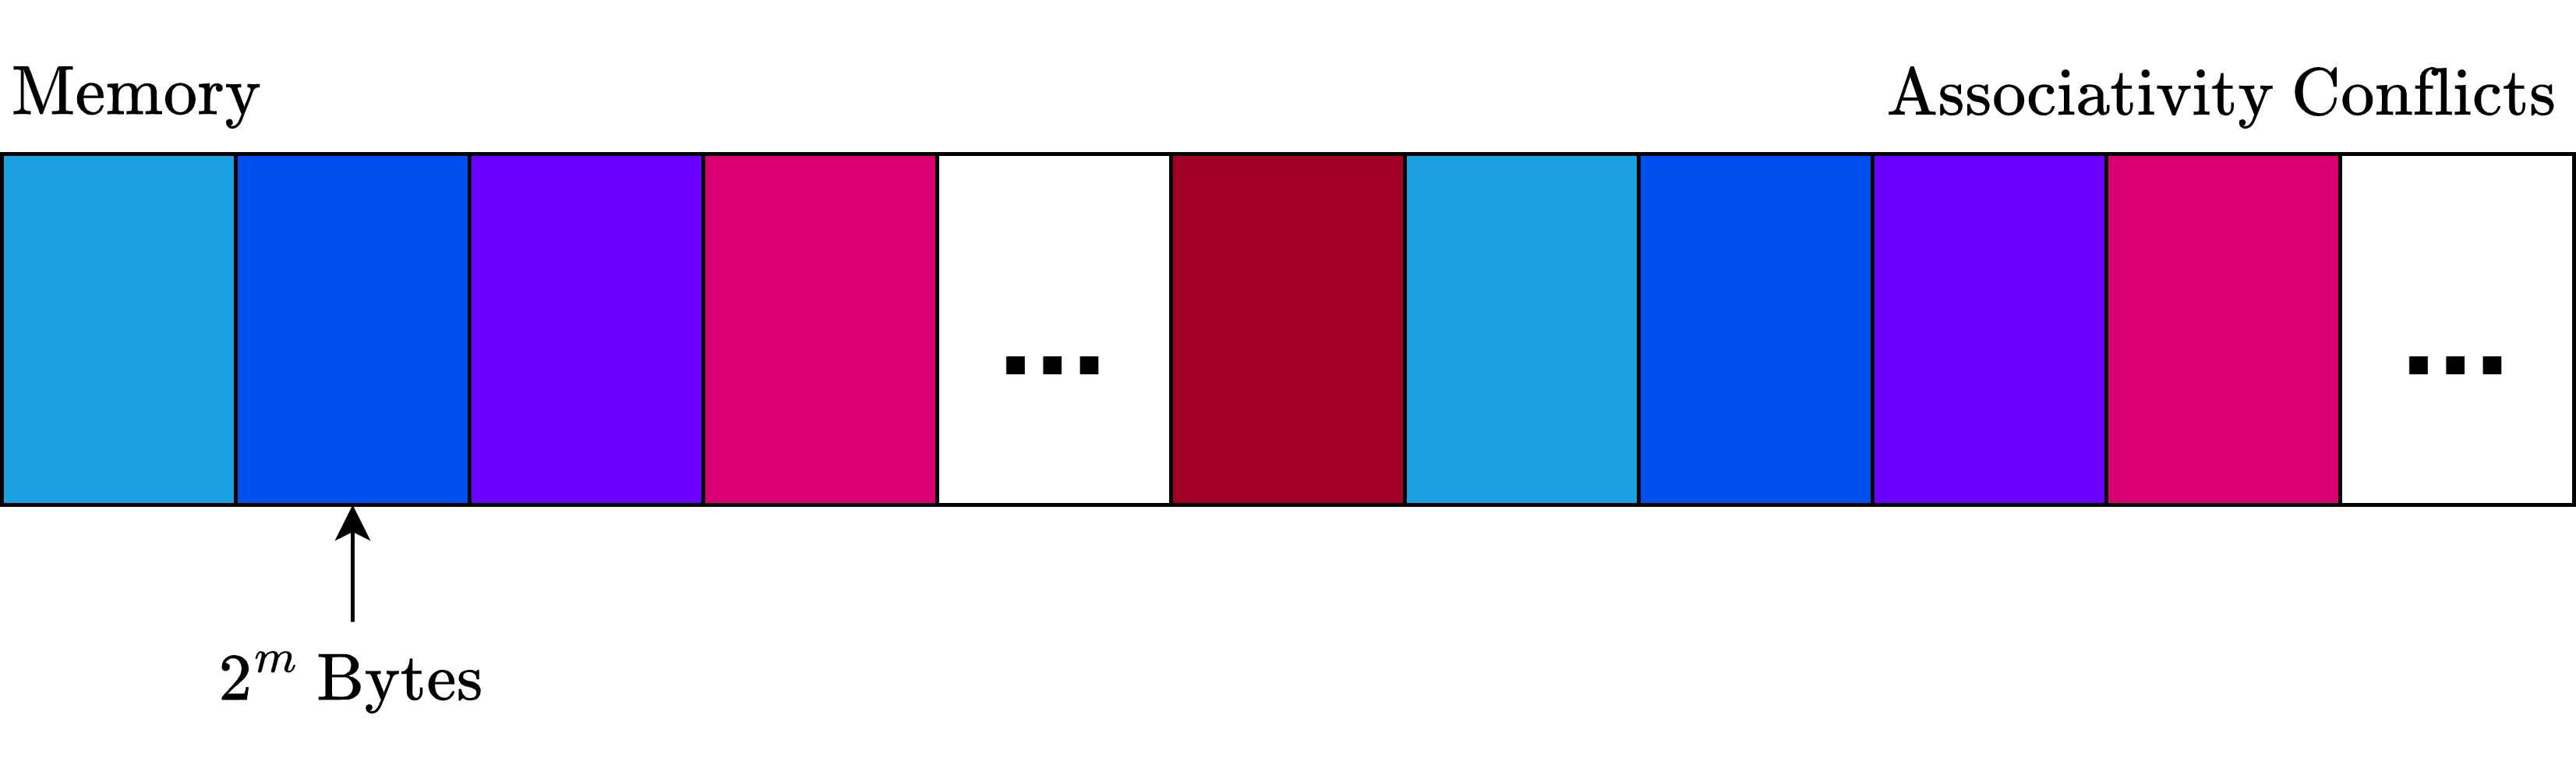
\includegraphics[width=.9\textwidth]{caches/images/associativity_conflicts.drawio.png}
\end{center}
\begin{prosbox}
    \begin{center}
        \begin{tabular}{r p{.8\textwidth}}
            \textbf{Simplicity} & Simple indexing of cache \& compare to determine hit/miss. \\
            \textbf{Fast Lookup} & Only one location where a cached value may be. \\
        \end{tabular}
    \end{center}
\end{prosbox}
\begin{consbox}
    \begin{center}
        \begin{tabular}{r p{.8\textwidth}}
            \textbf{Associativity Conflicts} & As location can only be cached in one place, associativity conflicts are common. \\
        \end{tabular}
    \end{center}
\end{consbox}

\subsection{Two Way Associative}
Combine two directly mapped caches, and only cache a given location in one.
\begin{center}
    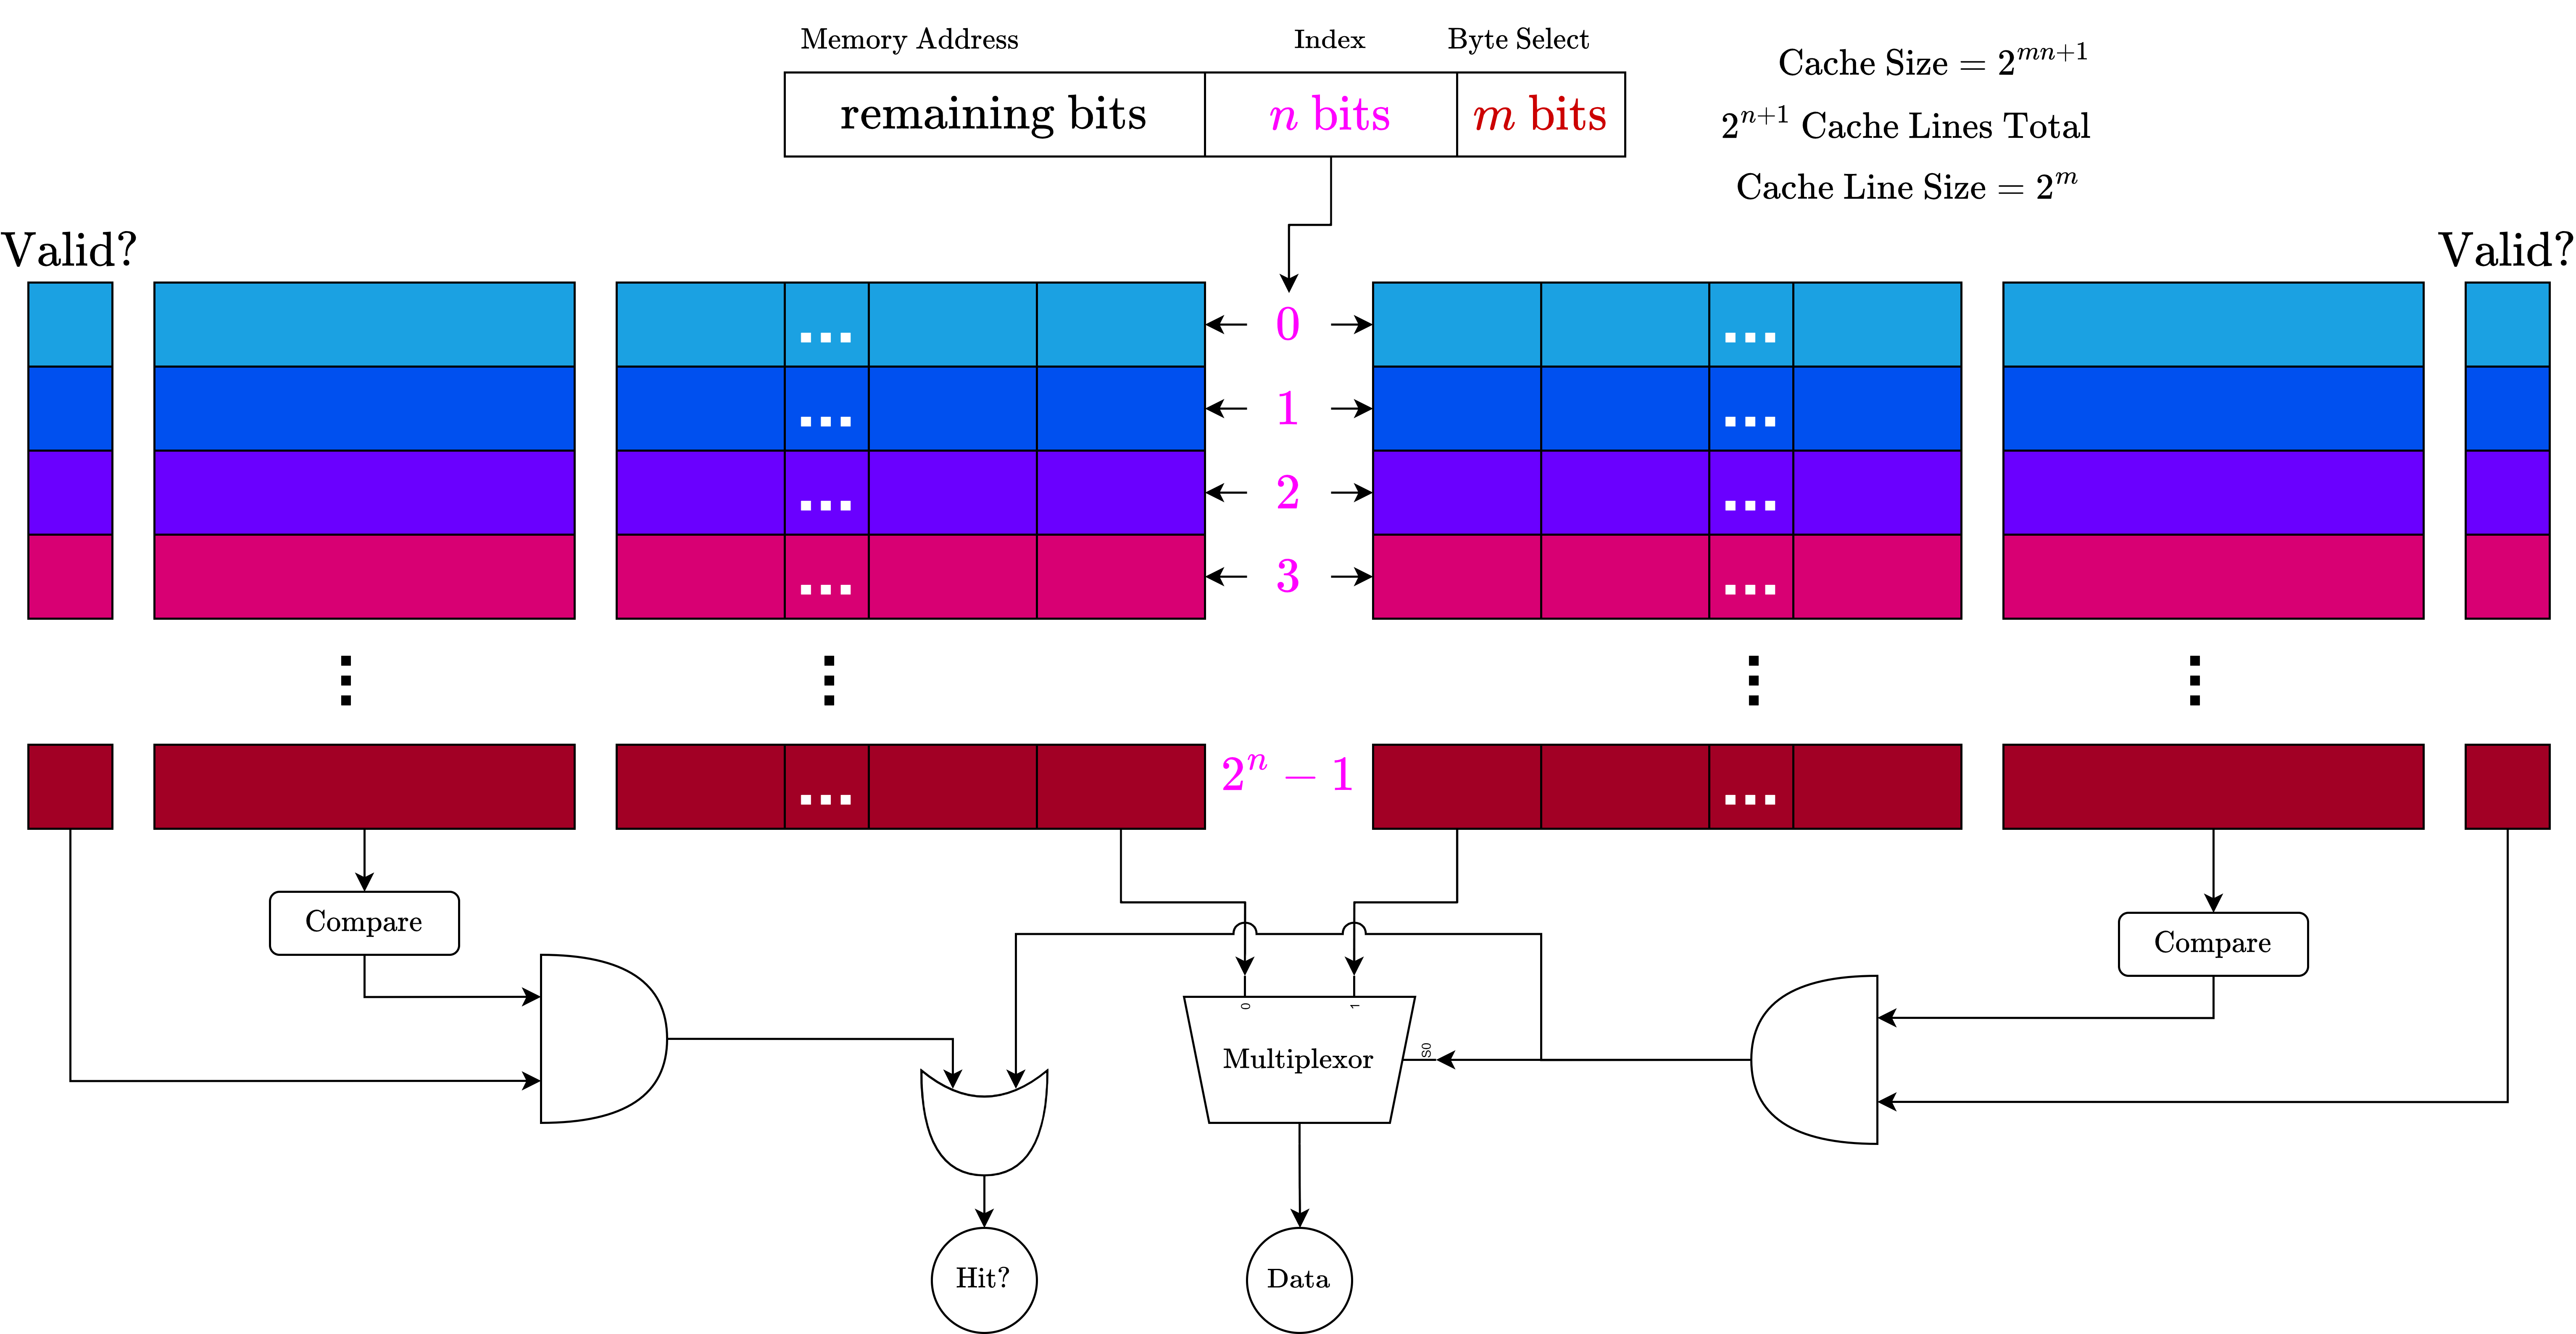
\includegraphics[width=.9\textwidth]{caches/images/two_way_set_associative.drawio.png}
\end{center}
\begin{itemize}
    \item Both caches searched in parallel.
    \item Only one hit possible, this is selected from result of both caches (selection is in the critical path)
    \item Cache block/line is available after the hit/miss is determined.
\end{itemize}

\begin{prosbox}
    \begin{center}
        \begin{tabular}{r p{.8\textwidth}}
            \textbf{Fewer Assoc Conflicts} & Any location can now select two different locations in the cache, hence two addresses with the same index can both be cached. \\
            \textbf{}
        \end{tabular}
    \end{center}
\end{prosbox}
\begin{consbox}
    \begin{center}
        \begin{tabular}{r p{.8\textwidth}}
            \textbf{Multiplexer Delay} & A multiplexer is added in the critical path \\
            \textbf{Complexity} & Requires more comparators, and more complexity in placement \& replacement. \\
        \end{tabular}
    \end{center}
\end{consbox}

\subsection{N Way Associative \& Block Placement}
A generalisation of the directly mapped and two way associative caches. Block placement is restricted by the cache's associativity.
\begin{itemize}
    \item Increasing associativity reduces associativity conflicts $\Rightarrow$ better hit rate (with diminishing returns)
    \item Greater overhead in terms of multiplexers in the critical path and the hardware complexity
    \item Fully associative cache can place any location in any cache location, and uses parallel search of tag (index is $0$ bits) to find entry
    \item More associative $\Rightarrow$ less sensitivity to storage layout
\end{itemize}
\begin{sidenotebox}{Intel Pentium 4 Level 1 Cache (pre-prescott)}
    \begin{center}
        \begin{tabular}{r l | r l}
            \textbf{Capacity:} & $8KB$ & \textbf{Block/Line Size:} & $64B$ so $\sfrac{8K}{64} = 128$ blocks\\
            \textbf{Ways/Associativity:} & $4$ & \textbf{Sets:} & $32$ ($128$ blocks, but $4$ way $\Rightarrow \sfrac{128}{4}$) \\
            \textbf{Index:} & $5$ bits & \textbf{Tag:} & $21$ bits \\
        \end{tabular}
    \end{center}
    Resulting access time is $2$ cycles ($6ns$ at $3GHz$), with cache/memory being dual ported (load and store).
\end{sidenotebox}

\section{Block Identification}
Index and tag identify a block.
\begin{itemize}
    \item Increasing associativity decreases index size, increases tag size.
    \item Increasing block size decreases index size.
\end{itemize}

\section{Block Replacement}
When introducing a new location to the cache \& possible locations are full.
\begin{itemize}
    \item No choice in directly mapped.
    \item $n$ choices for $n$-way associative.
\end{itemize}
The least recently used (LRU) evicts the oldest cache entry
\begin{itemize}
    \item In practice only a marginal advantage over random eviction.
    \item Can be pathologically bad (e.g a loop accessing many locations may evict the first just before restarting the loop \& accessing again).
\end{itemize}

\section{Write Strategy}
\begin{tcbraster}[raster columns=2, raster equal height]
    \begin{definitionbox}{Write Through}
        Write to cache, and to the block in lower-level memory.
        \begin{itemize}
            \item Combined with write buffers to prevent a wait on memory
        \end{itemize}
    \end{definitionbox}
    \begin{definitionbox}{Write Back}
        Only write back when evicting from cache. 
        \begin{itemize}
            \item Track write backs with a dirty bit
            \item Absorb cost of repeated writes
        \end{itemize}
    \end{definitionbox}
\end{tcbraster}
Neither avoid the cache-coherence problem (inconsistent values for locations cached on multiple cores/processors).

\section{Miss Rate Reduction Using Hardware}
\[\text{Average Memory Access Time (AMAT)} = \text{Hit Time} + \text{Miss Rate} \times \text{Miss Penalty}\]
In order to reduce AMAT:
\begin{itemize}
    \item Reduce Miss Rate.
    \item Reduce Miss Penalty.
    \item Reduce time to hit cache.
\end{itemize}

\subsection{Reducing Misses}
\begin{center}
    \begin{tabular}{l p{.8\textwidth}}
        \textbf{Compulsory} & First access so not in cache, also called a \textit{cold start miss} or \textit{first reference miss}. \\
        \textbf{Capacity} & Cache cannot contain all blocks needed during the execution of a program. A capacity miss occurs when a block discarded due to capacity is later retrieved. \\
        \textbf{Conflict} & Where the block placement strategy results in blocks being discarded as too many are mapped to a set (associativity conflicts). Also called \textit{collision misses} or \textit{interference misses}. \\
    \end{tabular}
\end{center}
\begin{center}
    \begin{tabular}{c c c}
        \textbf{Compulsory} & \textbf{Capacity} & \textbf{Conflict} \\
        Infinite Cache & Fully associative, finite cache & $n$-way associative, finite cache \\
    \end{tabular}
\end{center}

\begin{sidenotebox}{Coherence Miss}
    A miss caused by cache coherence protocols. For example another core or an I/O device may invalidate a cache entry. 
\end{sidenotebox}

\subsection{Increase Block Size}
\begin{tabbox}{prosbox}
    \textbf{Spatial Locality} & Larger block means more locations are speculatively cached. \\
    \textbf{Cold Misses} & As more speculatively cached, fewer cold misses (cached speculatively before first access). \\
\end{tabbox}
\begin{tabbox}{consbox}
    \textbf{Wasted Space} & More of the cache is wasted on speculatively cached but unused data. \\
    \textbf{Conflicts} & larger Blocks $\Rightarrow$ Fewer lines $\Rightarrow$ increase capacity conflicts as there is potentially more contention over lines. \\
    \textbf{Loading} & Larger blocks may take longer to load (increased miss penalty) or require a wider bus (expensive hardware). \\
\end{tabbox}

\subsection{Increase Associativity}

\begin{tabbox}{prosbox}
    \textbf{Fewer Associativity Conflicts} & More ways $\Rightarrow$ more ways to not conflict. This reduces the miss rate.\\
\end{tabbox}
\begin{tabbox}{consbox}
    \textbf{Cycle Time} & Comparators in the critical path
\end{tabbox}

\subsection{Victim Cache}
The main cache is a large directly mapped cache. A victim cache is fully associative and smaller, and contains data discarded from the main cache.
\begin{itemize}
    \item Checked in parallel.
    \item Rarely used for L1 cache, but often used for last-level caches.
\end{itemize}
This is an example of combining two strategies to avoid both's worst case behaviour.
\begin{sidenotebox}{Competitive Algorithms}
    Given two strategies, combining to create a good composite strategy.
    \begin{itemize}
        \item \href{https://en.wikipedia.org/wiki/Ski_rental_problem}{Ski Rental Problem} (Combining the renting \& buying strategies)
        \item Spinlocks vs context-switching (e.g spin before blocking?)
        \item Paging (replacement \& eviction)
        \item 
    \end{itemize}
\end{sidenotebox}

\subsection{Skewed-Associative Caches}
Given a two way set-associative cache.
\begin{itemize}
    \item Use a different \textit{hash function} for each cache (e.g one using regular (tag and index), other xors bits of index \& tag and reorders)
    \item Associativity conflicts may be present in one cache, but not the other.
\end{itemize}
\begin{center}
    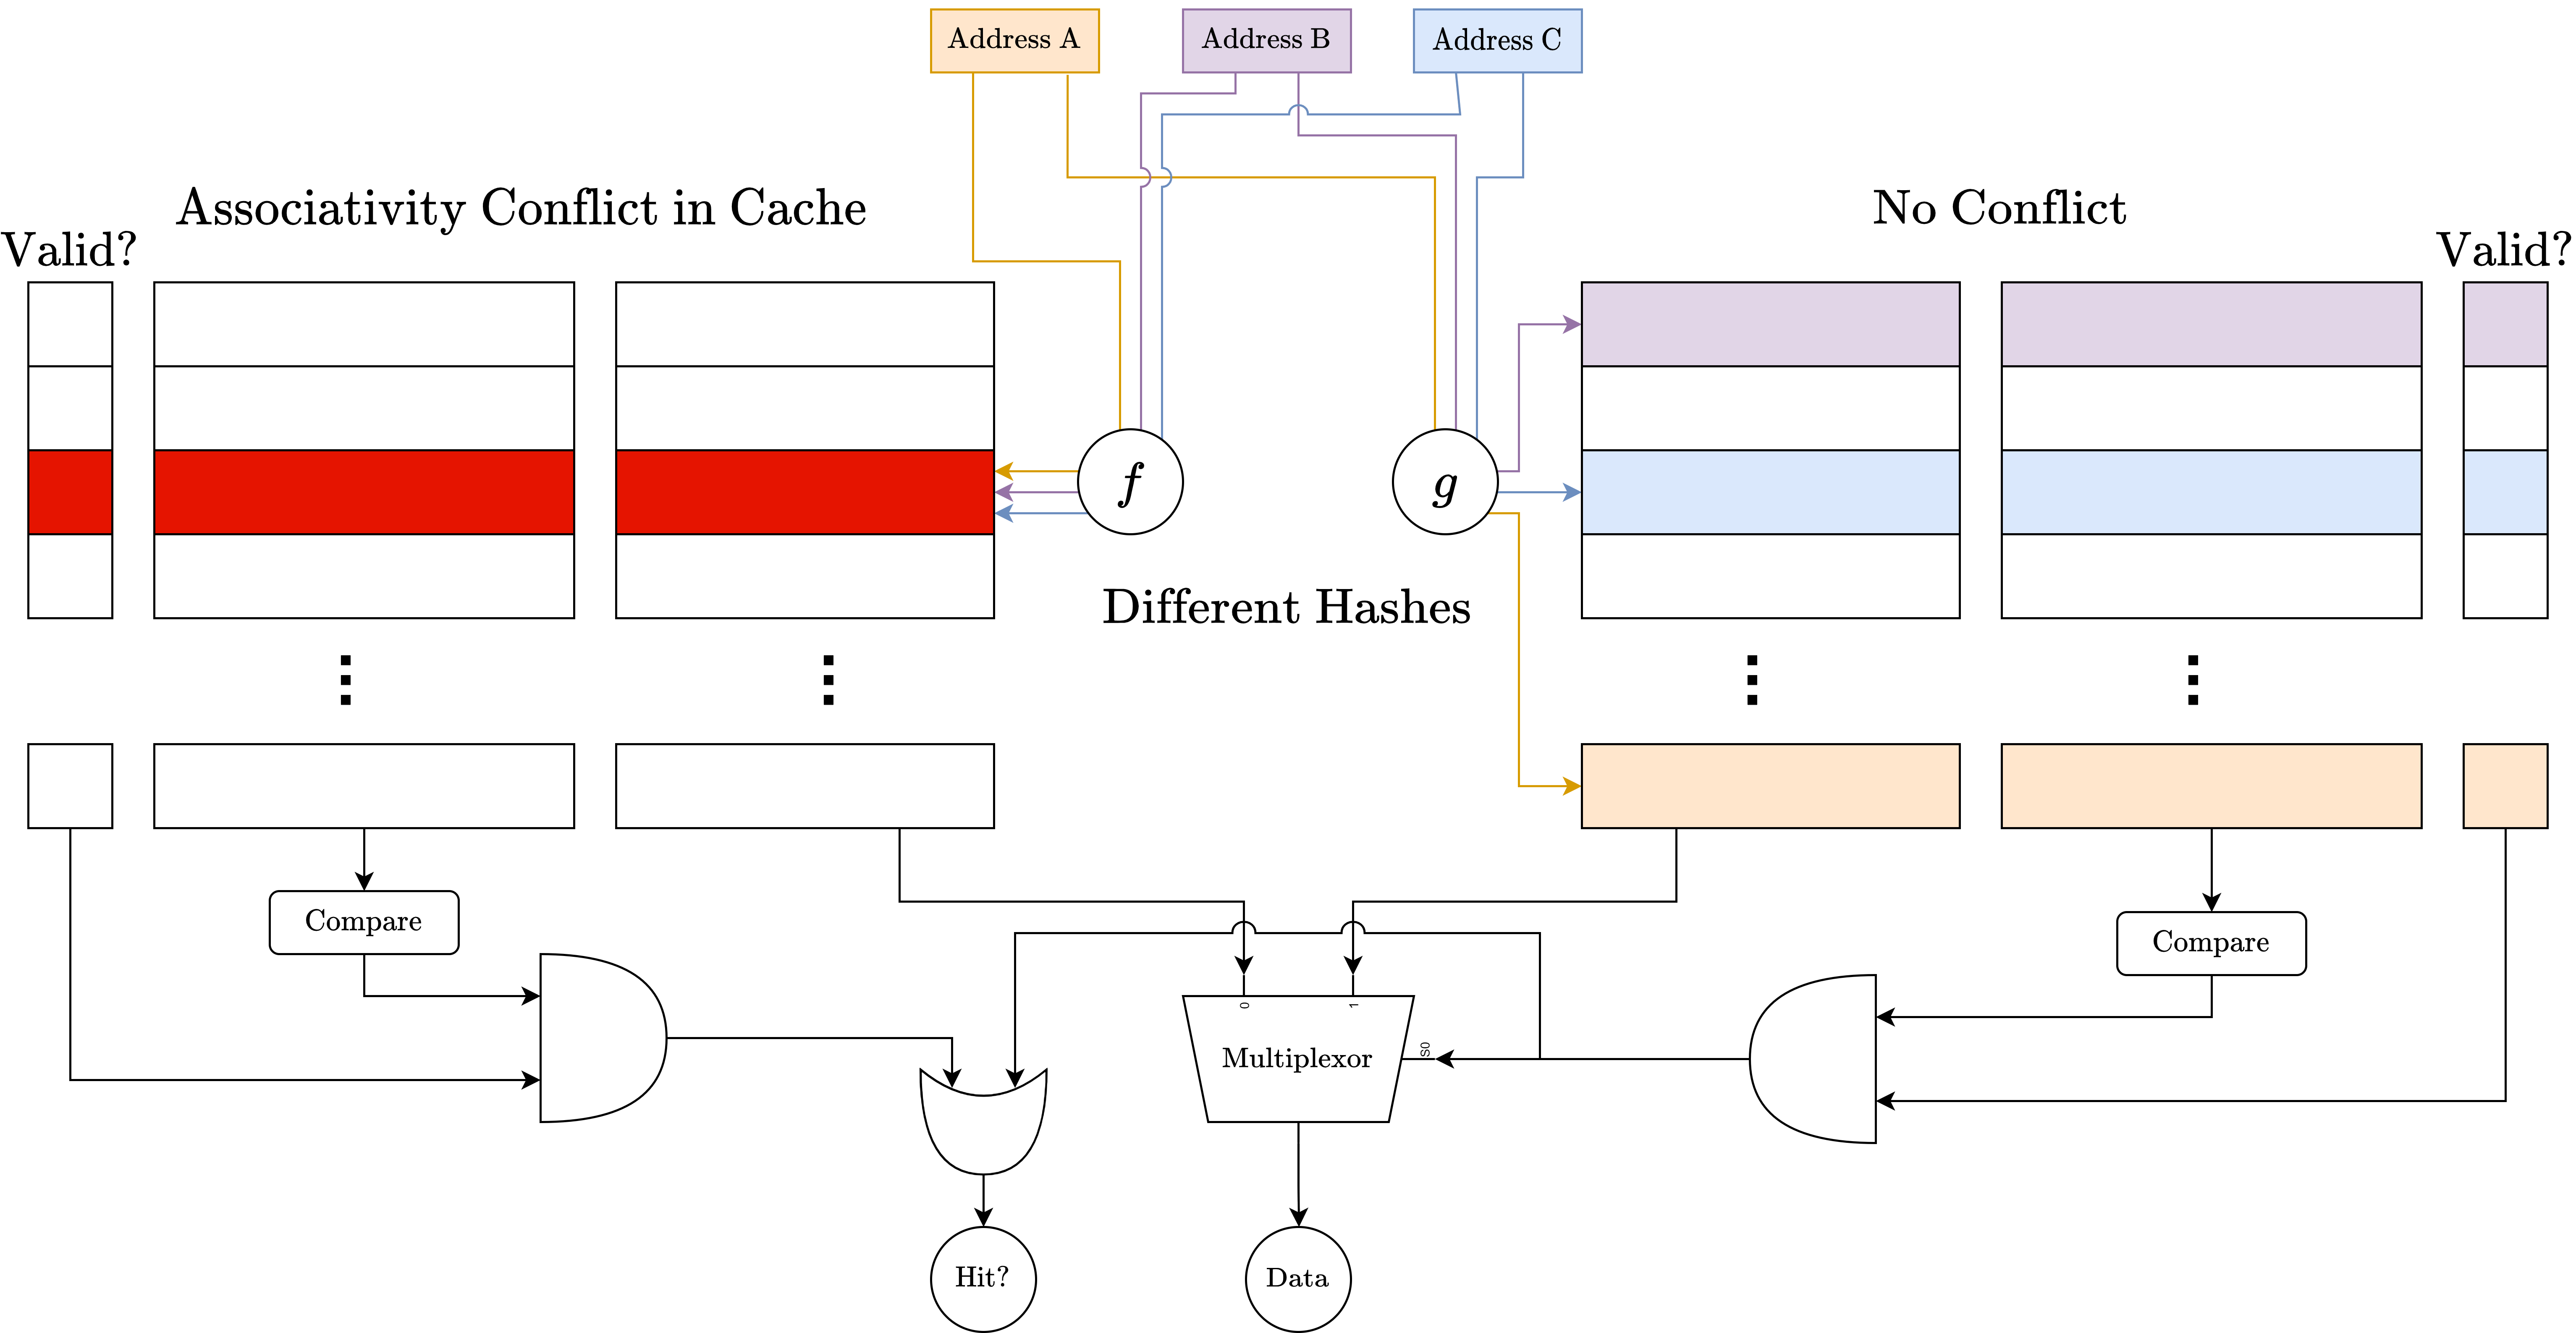
\includegraphics[width=.9\textwidth]{caches/images/skew_associative_cache.drawio.png}
\end{center}
\begin{tabbox}[.6\textwidth]{prosbox}
    \textbf{Associativity Conflicts} & Can reduce associativity conflicts. \\
    \textbf{Reduce Associativity} & Fewer conflicts for a w-way set associativity means the same conflict rate can be achieved with lower associativity (less hardware complexity). \\
    \textbf{More Predictable Average} & e.g with traversing two arrays and a non-skewed cache if we are \textit{"unlucky"} and get an associativity conflict on one element, we will get it on all subsequent. With skewed the next element may not. \\
\end{tabbox}
\begin{tabbox}{consbox}
    \textbf{Some Conflicts} & Its very difficult to write a program free of all conflicts. \\
    \textbf{More Decoders} & Need an address decoder per way/cache rather than a single for all. \\
    \textbf{Hash Latency} & Complex hash increases latency (it is in the critical path). \\
    \textbf{LRU} & Difficult to implement LRU eviction policy (though this is not necessarily a good policy). \\
\end{tabbox}

\subsection{Hardware Prefetching}
When a cache miss occurs, fetch the data (as required), but also pre-buffer the next block in a \textit{stream buffer}.
\begin{itemize}
    \item Prefetched blocks are placed in the cache (would pollute and potentially evict blocks to be used).
    \item Stream buffer checked in parallel with cache.
    \item Can add several prefetch buffers (multi-way stream buffer) to prefetch up $w$-way, fetch to $w$ blocks ahead.
    \item Used in most high performance processors.
\end{itemize}

\begin{tabbox}{prosbox}
    \textbf{Sequential Access} & Can avoid misses when traversing arrays. \\
    \textbf{Cache Untouched} & Can use any type of cache design with this - an addition. \\
\end{tabbox}

\begin{tabbox}[.7\textwidth]{consbox}
    \textbf{Memory Bandwidth} & Need extra bandwidth to transfer block selected (cache miss) and block for pre-fetch. \\
\end{tabbox}

\begin{sidenotebox}{Decoupled Access-Execute}
    Decouple the processor into an access and execution sides.
\begin{itemize}
    \item Access side fetches data to provide to the execute side.
    \item Execute side takes data from access and runs arithmetic instructions on it.
    \item Access side can be far ahead of execute, streaming the required data to it at close to memory bandwidth.
\end{itemize}
\end{sidenotebox}

\section{Miss Rate Reduction Using Software}
\subsection{Software Prefetching}
Many modern processors provide prefetching instructions.
\begin{itemize}
    \item Rarely needed - hardware prefetching is good!
    \item Useful on simpler processors with less or no hardware prefetching.
    \item Care required to prevent unwanted side effects.
    \item Prefetch instructions may target addresses that result in a page fault/protection violation (here they silently fail).
\end{itemize}

\subsection{Reducing Instruction Cache Misses}
Associativity conflicts can occur in the instruction cache.
\begin{itemize}
    \item We want to avoid hot loops calling functions who's code have an associativity conflict with eachother.
    \item By using the caller graph, with each loop labelled, we can determine how to pack subroutines into the program binary to avoid associativity conflicts.
    \item Needs to consider the entire program, and the layout of all subroutines so must be done at link-time.
\end{itemize}


\subsection{Storage Layout \& Iteration Space Transformations}
\begin{center}
    \begin{tabular}{l p{.7\textwidth}}
        \textbf{Merging Arrays} & Improve spatial locality by merging two arrays into a single array of compound elements (i.e a zip). (Struct of Arrays vs Array of Structs) \\
        \textbf{Multidimensional Array Permutation} & Match array layout to traversal order. \\
        \textbf{Loop Interchange} & Change nesting of loops to access data in order stored in memory. \\
        \textbf{Loop Fusion} & Combine independent loops that have the looping behaviour (e.g bounds) and overlapping variables. Sometimes this can then enable \textit{Array Contraction}, where some array can be replaced by a scalar value. \\
        \textbf{Blocking} & Improve temporal locality by accessing cache line sized blocks of data repeatedly instead of accessing columns or rows. \\
    \end{tabular}
\end{center}

\begin{definitionbox}{Morton Ordering}
    A traversal order for blocks.
    \begin{itemize}
        \item Split blocks into four.
        \item Traverse four blocks in $Z$ shape, recursively.
        \item A texture caching layout used in some GPUs.
    \end{itemize}
    \begin{minted}{Haskell}
data QuadTree a = Single a | 
  Quad { 
    topLeft :: QuadTree a, topRight :: QuadTree a, 
    bottomLeft :: QuadTree a, bottomRight :: QuadTree a
  }

{-
 A----->B
        |
 -------
 |
 C----->D
-}

morton :: (a -> b) -> (b -> b -> b -> b -> b) -> QuadTree a -> b
morton fun collect (Quad {tL, tR, bL, br}) 
  = collect (morton' tL) (morton' tR) (morton' bL) (morton' bR) 
  where
    morton' :: QuadTree a -> b
    morton' = morton fun collect
morton fun _ (Single s) = fun s
    \end{minted}
\end{definitionbox}
